\documentclass[aspectratio=169]{beamer}

% --- THEME AND STYLING ---
\usetheme{Madrid}
\useoutertheme{default}
\useinnertheme{rectangles}
\setbeamertemplate{navigation symbols}{}

% --- CUSTOM COLOR PALETTE ---
\definecolor{SkyBlue}{RGB}{135, 206, 235}
\definecolor{DarkNavy}{RGB}{0, 0, 139}
\definecolor{LightBlueBg}{RGB}{240, 248, 255}
\definecolor{AccentBlue}{RGB}{70, 130, 180}
\definecolor{DarkGreyText}{RGB}{50, 50, 50}
\definecolor{HighlightGreen}{RGB}{34, 139, 34}
\definecolor{AlertRed}{RGB}{220, 20, 60}

\setbeamercolor{palette primary}{bg=SkyBlue,fg=DarkNavy}
\setbeamercolor{palette secondary}{bg=DarkNavy,fg=white}
\setbeamercolor{palette tertiary}{bg=AccentBlue,fg=white}
\setbeamercolor{palette quaternary}{bg=SkyBlue,fg=DarkNavy}
\setbeamercolor{structure}{fg=DarkNavy}
\setbeamercolor{section in toc}{fg=DarkNavy}
\setbeamercolor{frametitle}{bg=SkyBlue,fg=DarkNavy}
\setbeamercolor{block title}{bg=DarkNavy,fg=white}
\setbeamercolor{block body}{bg=LightBlueBg,fg=DarkGreyText}
\setbeamercolor{block title alerted}{bg=AlertRed,fg=white}
\setbeamercolor{block body alerted}{bg=LightBlueBg,fg=DarkGreyText}
\setbeamercolor{block title example}{bg=HighlightGreen,fg=white}
\setbeamercolor{block body example}{bg=LightBlueBg,fg=DarkGreyText}
\setbeamertemplate{footline}[frame number]
\setbeamercolor{footline}{fg=DarkNavy}
\setbeamertemplate{blocks}[rounded][shadow=false]

% --- PACKAGES ---
\usepackage[utf8]{inputenc}
\usepackage{amsmath,amssymb}
\usepackage{booktabs}
\usepackage{graphicx}
\usepackage{array}
\usepackage{multirow}
\usepackage{tikz}
\usepackage{siunitx}

% --- TITLE PAGE ---
\title[Sustainable Rendezvous]{Sustainable ``Rendezvous'': A Festival Systems Challenge}
\subtitle{Comprehensive Process Optimization (Modules 3.1\,--\,3.4)}
\author[Team Sustainability]{Sustainability Task Force}
\institute{Department of Chemical Engineering\\
\vspace{0.2cm}
\small Course: CLL782 -- Process Optimization\\
\small Instructor: Prof.\ Om Prakash}
\date{\today}

\begin{document}

% ================================================================
%  TITLE
% ================================================================
\begin{frame}[plain]
    \titlepage
    \vspace{-0.5cm}
    \begin{center}
        \small Presented by: Yash
    \end{center}
\end{frame}

% ================================================================
%  OUTLINE
% ================================================================
\begin{frame}{Outline}
    \tableofcontents[hideallsubsections]
\end{frame}

% ================================================================
\section{1. The Genesis \& Vision}
% ================================================================

\begin{frame}{The Genesis: From Biodiversity to Urban Chaos}
    \begin{columns}[T]
        \begin{column}{0.6\textwidth}
            \begin{block}{The Inspiration}
                Sanskruti, General Secretary (Cultural Affairs), hails from the biodiverse landscapes of \textbf{West Champaran, Bihar}.
                \begin{itemize}
                    \item \textbf{Observation}: Urban life offers convenience but at a massive, silent environmental cost.
                    \item \textbf{The Trigger}: ``Rendezvous'' (Asia's Largest Fest) generates \textbf{tons of waste}, acting as a microcosm of urban un-sustainability.
                \end{itemize}
            \end{block}

            \begin{alertblock}{The Vision}
                \textit{``Sustainability is not about restriction, but about acting responsibly and optimizing resources.''}

                Transform Rendezvous from a logistical challenge into a \textbf{Model of Sustainability}.
            \end{alertblock}
        \end{column}

        \begin{column}{0.35\textwidth}
            \begin{exampleblock}{The Objective}
                Use \textbf{Systems Engineering \& Optimization} to:
                \begin{enumerate}
                    \item Quantify Impact.
                    \item Optimize Infrastructure.
                    \item Minimize Waste.
                \end{enumerate}
            \end{exampleblock}
        \end{column}
    \end{columns}
\end{frame}

\begin{frame}{Scope: The High-Intensity Zone}
    \begin{columns}[T]
        \begin{column}{0.55\textwidth}
            To ensure impact, we focus on the festival's core activity hub.

            \begin{table}
                \centering\small
                \begin{tabular}{l l}
                    \toprule
                    \textbf{Parameter} & \textbf{Value} \\ \midrule
                    Total Campus & 320 Acres \\
                    \textbf{Target ROI} & \textbf{82 Acres} (26\%) \\
                    Key Venues & OAT, Nalanda, SAC, LHC \\
                    Peak Footfall & $\sim$40{,}000/day \\
                    Grid System & 137 Cells ($\approx$0.6 ac) \\
                    Total (4 Days) & $\sim$160{,}000 attendees \\
                    \bottomrule
                \end{tabular}
            \end{table}
        \end{column}
        \begin{column}{0.40\textwidth}
            \centering
            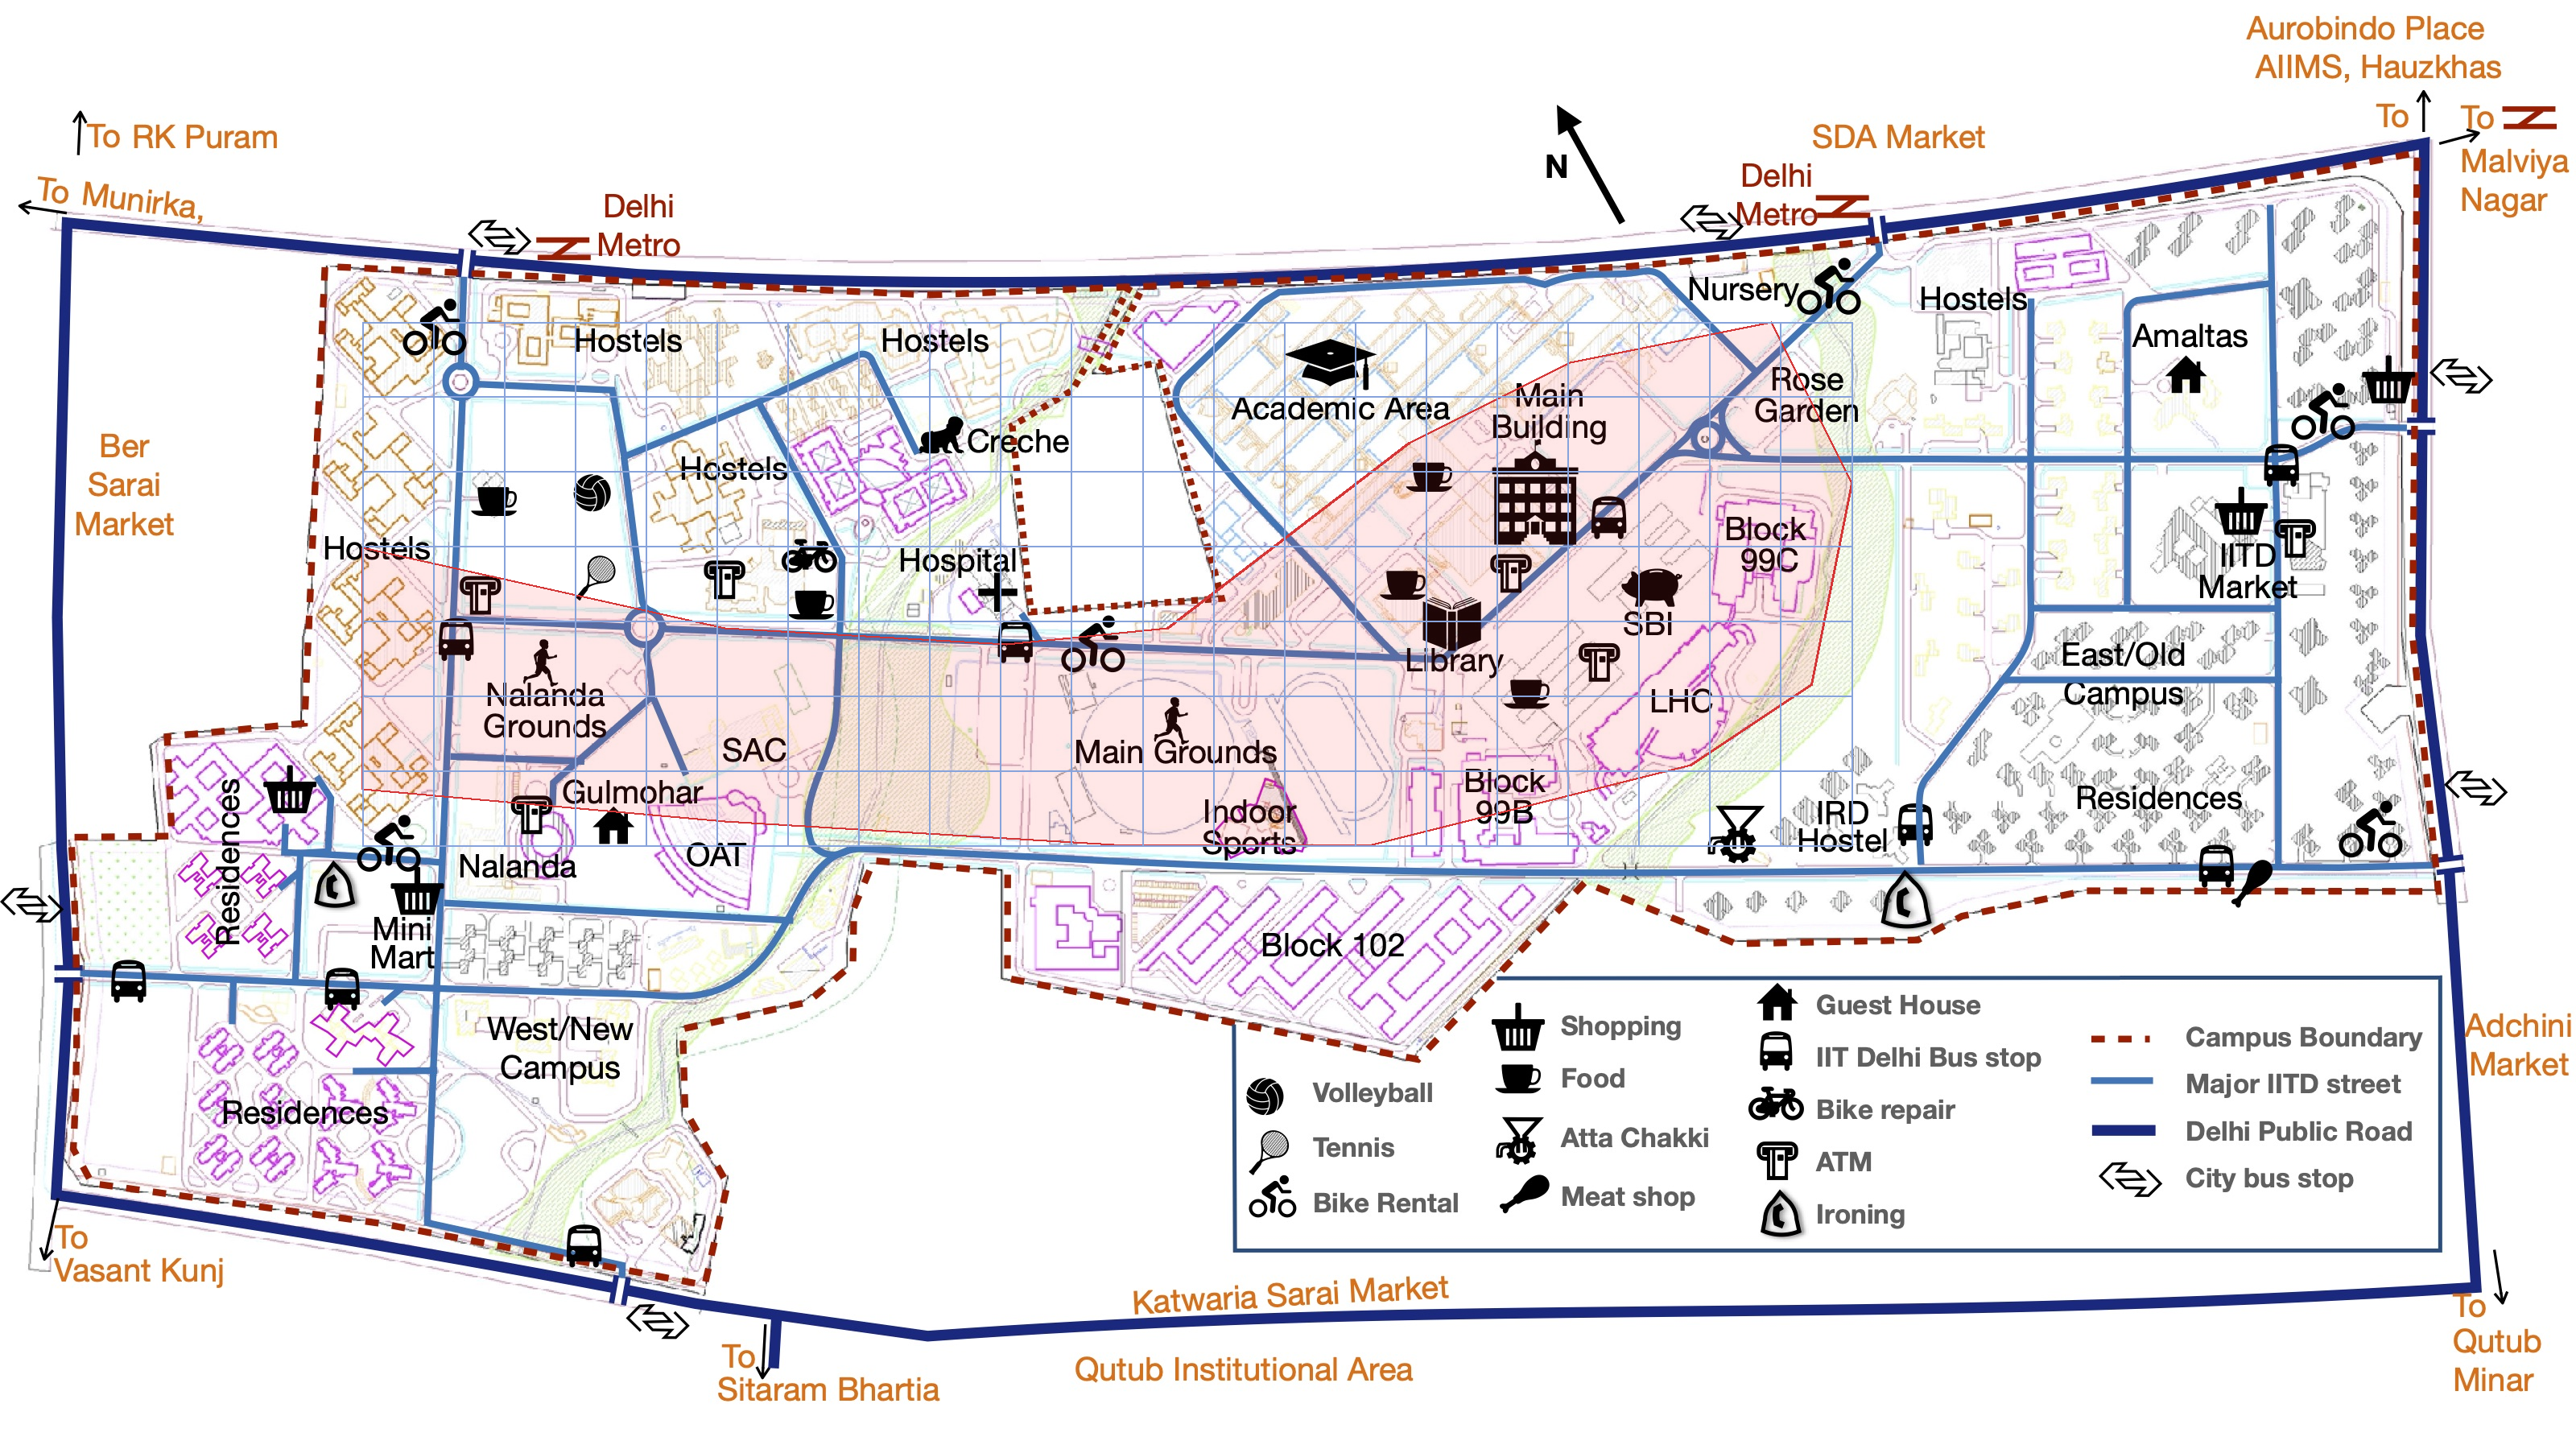
\includegraphics[width=0.95\textwidth]{../Module_3_1/iitd_roi_grid_map.jpg} \\
            \tiny{Figure: ROI with 137 Grid Cells overlaid on IITD Campus Map}
        \end{column}
    \end{columns}
\end{frame}

% ================================================================
\section{2. Module 3.1: Environmental Load}
% ================================================================

% --- Slide 1/4 ---
\begin{frame}{3.1 Problem Statement}
    \begin{block}{Objective}
        Define an environmental impact function $E = f(N, S, A)$ that quantifies the \textbf{total ecological footprint} of the festival --- incorporating energy use, waste generation, and emissions --- and find the conditions that \textbf{minimize} $E$.
    \end{block}

    \vspace{0.3cm}
    \textbf{Key Questions Addressed:}
    \begin{itemize}
        \item Can we capture non-linear phenomena like \textbf{crowding effects} and \textbf{diminishing returns}?
        \item What is the \textbf{ideal event scale} (stalls, hours) that minimizes footprint?
        \item Does the objective function need modification to better capture the sustainable festival design?
    \end{itemize}
\end{frame}

% --- Slide 2/4 ---
\begin{frame}{3.1 Variables \& Assumed Constants}
    \begin{table}
        \caption{Module 3.1 --- Variables and Parameters}
        \centering\footnotesize
        \begin{tabular}{l p{4.8cm} l l}
            \toprule
            \textbf{Symbol} & \textbf{Description} & \textbf{Unit} & \textbf{Type} \\ \midrule
            $N$ & Number of attendees & Persons & \textbf{Decision Var} \\
            $S$ & Number of food stalls & Stalls & \textbf{Decision Var} \\
            $A$ & Activity duration (concerts, events) & Activity-hrs & \textbf{Decision Var} \\
            $E$ & Total environmental load & kg CO$_2$-eq & Objective \\
            \midrule
            $\alpha_1$ & Per-capita base impact & 2.5 kg/p & Constant \\
            $\alpha_2$ & Per-stall embodied energy impact & 18 kg/stall & Constant \\
            $\alpha_3$ & Per-activity base impact & 12 kg/act-hr & Constant \\
            $\beta_N$ & Crowding nonlinearity coeff.\ (exp.~1.3) & 0.002 & Constant \\
            $\beta_S$ & Stall scaling nonlinearity coeff.\ (exp.~1.2) & 0.5 & Constant \\
            $\beta_A$ & Activity scaling coeff.\ (exp.~0.8) & 5.0 & Constant \\
            $\gamma_{NS}$ & Congestion penalty coefficient & 0.0005 & Constant \\
            \bottomrule
        \end{tabular}
    \end{table}

    \footnotesize \textbf{Ref:} Bettencourt et al.\ (2007) for $N^{1.3}$ scaling; CPCB (2021) for waste norms; CEA (2024) for grid emission.
\end{frame}

% --- Slide 3/4 ---
\begin{frame}{3.1 Mathematical Formulation}
    \begin{alertblock}{Environmental Load Function}
        $$ E = \underbrace{(\alpha_1 N + \alpha_2 S + \alpha_3 A)}_{\text{Base Load}} + \underbrace{(\beta_N N^{1.3} + \beta_S S^{1.2} + \beta_A A^{0.8})}_{\text{Non-linear Scaling}} + \underbrace{\left( \gamma_{NS} \frac{N^2}{S} \right)}_{\text{Congestion Penalty}} $$
    \end{alertblock}

    \textbf{Component Interpretation:}
    \begin{itemize}
        \item \textbf{Base Load} ($\alpha_1 N + \alpha_2 S + \alpha_3 A$): Direct consumption proportional to attendees, infrastructure, and activities.
        \item \textbf{Non-linear Scaling}:
            \begin{itemize}
                \item $\beta_N N^{1.3}$: Super-linear crowding --- more people $\Rightarrow$ disproportionately more littering (Urban Scaling Law).
                \item $\beta_S S^{1.2}$: Supply-chain fragmentation with increasing stalls.
                \item $\beta_A A^{0.8}$: Economies of scale in activities (Six-Tenths Rule).
            \end{itemize}
        \item \textbf{Congestion Penalty} ($N^2/S$): The critical ``queue'' term.
            \begin{itemize}
                \item Too few stalls ($S \downarrow$) $\Rightarrow$ Long queues $\Rightarrow$ Frustration \& Littering ($E \uparrow\uparrow$).
                \item Too many stalls ($S \uparrow$) $\Rightarrow$ Wasted embodied energy ($\alpha_2 S \uparrow$).
            \end{itemize}
    \end{itemize}
\end{frame}

% --- Slide 4/4 ---
\begin{frame}{3.1 Optimization \& Insights}
    \begin{exampleblock}{Optimal Stall Count (Fixed $N$)}
        Differentiating $E$ w.r.t.\ $S$ and setting to zero:
        $$ \frac{\partial E}{\partial S} = \alpha_2 + 1.2\,\beta_S\,S^{0.2} - \gamma_{NS} \frac{N^2}{S^2} = 0 $$
        Approximating for small $\beta_S$ ($\beta_S \approx 0$):
        $$ \alpha_2 \approx \gamma_{NS} \frac{N^2}{S^2} \implies \boxed{S^* \approx N \sqrt{\frac{\gamma_{NS}}{\alpha_2}}} $$
    \end{exampleblock}

    \begin{columns}[T]
        \begin{column}{0.48\textwidth}
            \textbf{Numerical Result ($N = 40{,}000$/day):}
            $$ S^* \approx 40000 \sqrt{\frac{0.0005}{18}} \approx \mathbf{210} $$
        \end{column}
        \begin{column}{0.48\textwidth}
            \textbf{Key Insights:}
            \begin{itemize}
                \item Current practice ($\sim$100 stalls) is \textbf{under-provisioned}.
                \item Congestion penalty \textbf{dominates} at low $S$.
                \item Increasing to $\sim$210 stalls paradoxically \textit{reduces} total $E$.
                \item Sublinear $A^{0.8}$ favors consolidating activities.
            \end{itemize}
        \end{column}
    \end{columns}
\end{frame}

% ================================================================
\section{3. Module 3.2: Dustbin Placement (FLP)}
% ================================================================

% --- Slide 1/4 ---
\begin{frame}{3.2 Problem Statement}
    \begin{block}{Objective}
        Formulate a \textbf{Facility Location Problem (FLP)} to optimally place dustbins across the 82-acre festival zone, minimizing average walking distance weighted by footfall density.
    \end{block}

    \vspace{0.3cm}
    \textbf{Key Considerations:}
    \begin{itemize}
        \item 3 Bin Types: \textbf{Recyclable}, \textbf{Compostable}, \textbf{General}.
        \item Each bin has a \textbf{cost}, a \textbf{service radius} $R_t$, and a \textbf{capacity} $K_t$.
        \item \textbf{Greenery Protection}: Bins on hardscape edges only (no trampling of lawns).
        \item Designed for \textbf{peak surge} demand (Star Night: 40{,}000 in the zone).
    \end{itemize}
\end{frame}

% --- Slide 2/4 ---
\begin{frame}{3.2 Variables, Constants \& Data}
    \begin{table}
        \caption{Module 3.2 --- Nomenclature}
        \centering\footnotesize
        \begin{tabular}{l p{4.8cm} l l}
            \toprule
            \textbf{Sym} & \textbf{Description} & \textbf{Unit} & \textbf{Type} \\ \midrule
            $y_{j,t}$ & Install bin type $t$ at location $j$? & $\{0,1\}$ & \textbf{Binary Decision} \\
            $a_{i,j,t}$ & Fraction of zone $i$ demand $\to$ bin $j$ & $[0,1]$ & Continuous Decision \\
            $F_i$ & Peak footfall at zone $i$ & Ppl/hr & Parameter \\
            $D_{ij}$ & Walking distance $i \to j$ & m & Parameter \\
            \midrule
            $w$ & Waste generation rate & 0.15 kg/p & Constant \\
            $R_t$ & Service radius & 30--50 m & Constant \\
            $K_t$ & Bin capacity (dual FRP) & 20--30 kg & Constant \\
            $C_t$ & Bin procurement cost & Rs.\,10--15K & Constant \\
            $B$ & Total budget & Rs.\ & Constraint \\
            \bottomrule
        \end{tabular}
    \end{table}

    \footnotesize \textbf{Ref:} Disney 30-ft rule; Glasdon bin-spacing norms (30--50 m); CPCB waste norms.
\end{frame}

% --- Slide 3/4 ---
\begin{frame}{3.2 Mathematical Formulation (MILP)}
    \begin{exampleblock}{Minimize Total User Inconvenience}
        $$ \text{Min } Z = \sum_{i=1}^{m} \sum_{j=1}^{p} \sum_{t} F_i \cdot a_{i,j,t} \cdot D_{ij} $$
    \end{exampleblock}

    \textbf{Subject to:}
    \begin{enumerate}
        \item \textbf{Coverage}: Every zone must be fully served.
            $\displaystyle\sum_{j,t} a_{i,j,t} = 1 \quad \forall\, i$
        \item \textbf{Logical Link}: No assignment without installation.
            $a_{i,j,t} \le y_{j,t} \quad \forall\, i,j,t$
        \item \textbf{Capacity}: Bins must not overflow.
            $\displaystyle\sum_{i} F_i \cdot w \cdot a_{i,j,t} \le K_t \cdot y_{j,t} \quad \forall\, j,t$
        \item \textbf{Accessibility}: $a_{i,j,t} = 0$ if $D_{ij} > R_t$
        \item \textbf{Budget}: $\displaystyle\sum_{j,t} C_t \cdot y_{j,t} \le B$
    \end{enumerate}
\end{frame}

% --- Slide 4/4 ---
\begin{frame}{3.2 Optimization Analysis \& Insights}
    \begin{columns}[T]
        \begin{column}{0.48\textwidth}
            \begin{block}{Complexity}
                \begin{itemize}
                    \item \textbf{NP-hard} Facility Location.
                    \item Discretize ROI into 20m $\times$ 20m grid.
                    \item Solvable via Branch-and-Bound (Gurobi / CBC).
                \end{itemize}
            \end{block}
        \end{column}

        \begin{column}{0.48\textwidth}
            \begin{alertblock}{Expected Outcomes}
                \begin{itemize}
                    \item \textbf{High density} near OAT/Amul (food zones, high $F_i$).
                    \item \textbf{Sparse} along Main Road (low $F_i$, $R_t$ constraint).
                    \item Relaxing binary $\to$ LP gives lower bound.
                \end{itemize}
            \end{alertblock}
        \end{column}
    \end{columns}

    \vspace{0.3cm}
    \textbf{Data Summary:}
    \begin{itemize}
        \item Total peak waste: $40{,}000 \times 0.15 = \mathbf{6{,}000}$ kg/day.
        \item At $K_t = 30$ kg/bin $\Rightarrow$ minimum $\sim$200 bins needed.
        \item Budget feasibility: 200 bins $\times$ Rs.\,12K $\approx$ Rs.\,24 Lakhs.
    \end{itemize}
\end{frame}

% ================================================================
\section{4. Module 3.3: Waste Collection Logistics}
% ================================================================

% --- Slide 1/4 ---
\begin{frame}{3.3 Problem Statement}
    \begin{block}{Objective}
        Design an efficient \textbf{waste collection and processing logistics} system that transports 6{,}000 kg/day of segregated waste from generation zones to processing facilities, minimizing total cost.
    \end{block}

    \vspace{0.3cm}
    \textbf{System Architecture:}
    \begin{itemize}
        \item \textbf{Sources} ($i$): Demand zones within the 82-acre ROI.
        \item \textbf{Sinks} ($j$): 3 Processing Facilities:
            \begin{enumerate}
                \item On-Campus Biogas/Compost ($\sim$1 km, Cap: 500 kg/day).
                \item Okhla Landfill/WTE ($\sim$12 km, Unconstrained capacity).
                \item Okhla Recycling Aggregator ($\sim$11 km, Net \textit{revenue}).
            \end{enumerate}
        \item \textbf{Fleet}: Electric Tippers (Tata Ace EV).
    \end{itemize}
\end{frame}

% --- Slide 2/4 ---
\begin{frame}{3.3 Variables, Constants \& Data}
    \begin{table}
        \caption{Module 3.3 --- Nomenclature}
        \centering\footnotesize
        \begin{tabular}{l p{4.8cm} l l}
            \toprule
            \textbf{Sym} & \textbf{Description} & \textbf{Unit} & \textbf{Type} \\ \midrule
            $x_{i,j}$ & Waste flow from zone $i$ to facility $j$ & kg & \textbf{Continuous Decision} \\
            $v_k$ & Deploy vehicle $k$? & $\{0,1\}$ & Binary Decision \\
            $W_i$ & Total waste at zone $i$ & kg & Parameter \\
            $D_{ij}$ & Distance zone $i$ to facility $j$ & km & Parameter \\
            \midrule
            $V_{cap}$ & Vehicle payload (Tata Ace EV) & 600--750 kg & Constant \\
            $C_{dist}$ & Transport cost per km & Rs.\,15--20/km & Constant \\
            $C_{handling}$ & Handling cost per kg & Rs./kg & Constant \\
            $C_{fixed}$ & Fixed cost per vehicle per day & Rs.\,500--800 & Constant \\
            $C_{proc,j}$ & Processing cost at facility $j$ & Rs./kg & Constant \\
            \bottomrule
        \end{tabular}
    \end{table}

    \footnotesize \textbf{Assumptions:} Direct transport (Star network); Homogeneous fleet; Linear costs.
\end{frame}

% --- Slide 3/4 ---
\begin{frame}{3.3 Formulation (Minimum Cost Flow)}
    \begin{alertblock}{Minimize Total Logistics Cost}
        $$ Z = \underbrace{\sum_{i,j} x_{i,j}\,(C_{dist}\,D_{ij} + C_{handling} + C_{proc,j})}_{\text{Variable Cost (Transport + Processing)}} + \underbrace{C_{fixed} \cdot \sum_{k} v_k}_{\text{Fixed Fleet Cost}} $$
    \end{alertblock}

    \textbf{Subject to:}
    \begin{enumerate}
        \item \textbf{Waste Clearance} (all waste removed):
            $\displaystyle\sum_{j} x_{i,j} = W_i \quad \forall\, i$
        \item \textbf{Facility Throughput}:
            $\displaystyle\sum_{i} x_{i,j} \le Cap_j \quad \forall\, j$
        \item \textbf{Fleet Capacity}:
            $\displaystyle\sum_{i,j} x_{i,j} \le V_{cap} \cdot \sum_{k} v_k$
        \item \textbf{Non-negativity}: $x_{i,j} \ge 0$, $v_k \in \{0,1\}$
    \end{enumerate}
\end{frame}

% --- Slide 4/4 ---
\begin{frame}{3.3 Sensitivity Analysis \& Insights}
    \begin{columns}[T]
        \begin{column}{0.48\textwidth}
            \begin{block}{Complexity}
                \begin{itemize}
                    \item Core: LP Transportation Problem (Totally Unimodular $\Rightarrow$ Polynomial).
                    \item Integer constraint on $v_k$ $\Rightarrow$ MILP, but single scalar $\Rightarrow$ very low complexity.
                \end{itemize}
            \end{block}
        \end{column}

        \begin{column}{0.48\textwidth}
            \begin{alertblock}{Sensitivity (+20\% Waste)}
                If $W'_i = 1.2\,W_i$:
                \begin{itemize}
                    \item Check: $\sum W'_i \le \sum Cap_j$?
                    \item Variable costs scale \textbf{linearly}.
                    \item But vehicle fixed cost has a \textbf{step-function} jump if fleet is saturated.
                \end{itemize}
            \end{alertblock}
        \end{column}
    \end{columns}

    \vspace{0.3cm}
    \textbf{Key Insights:}
    \begin{itemize}
        \item \textbf{Waste Composition}: 40\% Organic, 40\% Recyclable, 20\% Inert (CPCB norms).
        \item \textbf{Bottleneck}: On-campus biogas (500 kg) saturates first $\Rightarrow$ overflow to landfill.
        \item \textbf{Revenue Opportunity}: Recycling aggregator provides net \textit{revenue} (Rs.\,5--10/kg) for segregated waste.
    \end{itemize}
\end{frame}

% ================================================================
\section{5. Module 3.4: Water Refill Stations}
% ================================================================

% --- Slide 1/4 ---
\begin{frame}{3.4 Problem Statement}
    \begin{block}{Objective}
        Plan \textbf{water refill station} locations using a \textbf{Capacitated P-Median} formulation. Minimize total cost (installation + user walking inconvenience) to support a reusable water bottle policy and \textbf{eliminate single-use plastic}.
    \end{block}

    \vspace{0.3cm}
    \textbf{Key Considerations:}
    \begin{itemize}
        \item Each participant receives a metallic bottle (cost recovered via festival pass).
        \item Stations can only be installed at \textbf{pre-designated feasible locations} (near existing plumbing).
        \item Demand is \textbf{splittable}: aggregate probability of users visiting nearby stations.
        \item Delhi climate $\Rightarrow$ high hydration need ($\sim$250 ml/hr/person).
    \end{itemize}
\end{frame}

% --- Slide 2/4 ---
\begin{frame}{3.4 Variables, Constants \& Data}
    \begin{table}
        \caption{Module 3.4 --- Nomenclature}
        \centering\footnotesize
        \begin{tabular}{l p{4.8cm} l l}
            \toprule
            \textbf{Sym} & \textbf{Description} & \textbf{Unit} & \textbf{Type} \\ \midrule
            $y_j$ & Install station at location $j$? & $\{0,1\}$ & \textbf{Binary Decision} \\
            $x_{i,j}$ & Fraction of zone $i$ served by $j$ & $[0,1]$ & Continuous Decision \\
            $d_i$ & Water demand at zone $i$ & Ppl/hr & Parameter \\
            $D_{ij}$ & Walking distance $i \to j$ & m & Parameter \\
            \midrule
            $f_j$ & Installation + operation cost & Rs.\,1 Lakh & Constant \\
            $cap_j$ & Station dispensing capacity & 250 LPH & Constant \\
            $C_{walk}$ & Monetary value of walking & Rs.\,0.02/m & Constant \\
            \bottomrule
        \end{tabular}
    \end{table}

    \footnotesize \textbf{Ref:} Blue Star/Voltas 150--300 LPH specs; WHO hydration norms; Market pricing (Indiamart).
    
    \vspace{0.2cm}
    \footnotesize \textbf{Peak Water Demand}: $40{,}000 \times 0.25$ L/hr = \textbf{10{,}000 LPH}. At 250 LPH/station $\Rightarrow$ Min.\ $\sim$40 stations.
\end{frame}

% --- Slide 3/4 ---
\begin{frame}{3.4 Formulation (Capacitated P-Median)}
    \begin{exampleblock}{Minimize Generalized Cost}
        $$ Z = \underbrace{\sum_{j=1}^{p} f_j\,y_j}_{\text{Installation (CAPEX)}} + \underbrace{\sum_{i=1}^{m}\sum_{j=1}^{p} \alpha_{ij}\,x_{i,j}}_{\text{User Inconvenience}} $$
        where $\alpha_{ij} = d_i \cdot D_{ij} \cdot C_{walk}$ is the weighted walking cost coefficient.
    \end{exampleblock}

    \textbf{Subject to:}
    \begin{enumerate}
        \item \textbf{Demand Satisfaction}: $\displaystyle\sum_{j} x_{i,j} = 1 \quad \forall\, i$
        \item \textbf{Station Capacity}: $\displaystyle\sum_{i} d_i\,x_{i,j} \le cap_j \cdot y_j \quad \forall\, j$
            \\ \footnotesize (Also acts as logical link: if $y_j = 0$, capacity is 0.)
        \item \textbf{Integrality}: $y_j \in \{0, 1\}$, \quad $0 \le x_{i,j} \le 1$
    \end{enumerate}
\end{frame}

% --- Slide 4/4 ---
\begin{frame}{3.4 Solution Strategy \& Insights}
    \begin{columns}[T]
        \begin{column}{0.48\textwidth}
            \begin{block}{Algorithmic Approach}
                \begin{enumerate}
                    \item \textbf{Greedy}: Iteratively add the station yielding max cost reduction.
                    \item \textbf{Lagrangian Relaxation}: Relax demand constraints; decompose into knapsack sub-problems.
                    \item \textbf{Exact}: Branch-and-Bound (Gurobi/CBC). With $m \approx 50$, $p \approx 20$: converges in seconds.
                \end{enumerate}
            \end{block}
        \end{column}

        \begin{column}{0.48\textwidth}
            \begin{alertblock}{Key Trade-offs}
                \begin{itemize}
                    \item High $f_j$ $\Rightarrow$ Fewer, centralized stations (long walks).
                    \item Low $f_j$ $\Rightarrow$ Distributed topology (short walks).
                    \item \textbf{Shadow Price} of capacity constraint reveals bottleneck stations to upgrade.
                \end{itemize}
            \end{alertblock}
        \end{column}
    \end{columns}

    \vspace{0.2cm}
    \textbf{Fairness Note:} Current objective minimizes \textit{average} distance. A \textbf{Minimax} secondary constraint could ensure no zone walks more than a threshold.
\end{frame}

% ================================================================
\section{Conclusion}
% ================================================================

\begin{frame}{Integrated Blueprint \& Next Steps}
    \begin{block}{System-Level Summary}
        \begin{enumerate}
            \item \textbf{Mod 3.1}: Right-size infrastructure ($S^* \approx 210$ stalls) to cut congestion-led waste.
            \item \textbf{Mod 3.2}: Place $\sim$200 bins within 30--50 m radius to capture waste at source.
            \item \textbf{Mod 3.3}: Route 6{,}000 kg/day via optimized fleet (minimize cost, maximize recycling revenue).
            \item \textbf{Mod 3.4}: Deploy $\sim$40 refill stations to eliminate single-use plastic.
        \end{enumerate}
    \end{block}

    \begin{exampleblock}{Module 3.5 (Next): System Integration}
        Combine all modules into a \textbf{multi-objective optimization}: minimize total cost \textit{and} environmental impact \textit{and} user inconvenience, subject to combined constraints from Modules 3.1--3.4.
    \end{exampleblock}
\end{frame}

\begin{frame}[plain]
    \vfill
    \begin{center}
        {\Huge \textcolor{DarkNavy}{Thank You}} \\
        \vspace{0.8cm}
        {\large \textit{``Just like Mother Nature, we optimize continuously ---}}\\
        {\large \textit{learning, adapting, and improving.''}}\\
        \vspace{0.8cm}
        \small Sustainable Rendezvous Project \\
        \small Dept.\ of Chemical Engineering, IIT Delhi
    \end{center}
    \vfill
\end{frame}

\end{document}
